\documentclass[12pt]{article}
\usepackage[margin=1in]{geometry}
\usepackage{graphicx}
\usepackage{amsmath}
\usepackage{tikz}
\usepackage{hyperref}
\usepackage{enumitem}

\newcommand{\fromlectures}{{\\ \color{blue} \hspace*{\fill}(from lecture slides)} \\}
\newcommand{\bydefn}{{\\ \color{blue} \hspace*{\fill}(by definition)} \\}
\newcommand{\given}{{\\ \color{blue} \hspace*{\fill}(given)} \\}
\newcommand{\rtp}{{\\ \color{blue} \hspace*{\fill}(required to prove)} \\}

\newcommand{\f}[1]{o_{#1}x_{#1}y_{#1}z_{#1}}
\newcommand{\rx}[1]{\begin{bmatrix} 1 & 0 & 0 & 0 \\ 0 & cos(#1) & -sin(#1) & 0 \\ 0 & sin(#1) & cos(#1) & 0 \\ 0 & 0 & 0 & 1 \end{bmatrix}}
\newcommand{\rz}[1]{\begin{bmatrix} cos(#1) & -sin(#1) & 0 & 0 \\ sin(#1) & cos(#1) & 0 & 0 \\ 0 & 0 & 1 & 0 \\ 0 & 0 & 0 & 1 \end{bmatrix}}
\newcommand{\iden}{\begin{bmatrix} 1 & 0 & 0 & 0 \\ 0 & 1 & 0 & 0 \\ 0 & 0 & 1 & 0 \\ 0 & 0 & 0 & 1 \end{bmatrix}}
\newcommand{\trans}[3]{\begin{bmatrix} 1 & 0 & 0 & #1 \\ 0 & 1 & 0 & #2 \\ 0 & 0 & 1 & #3 \\ 0 & 0 & 0 & 1 \end{bmatrix}}

\title{CSci 5551 - HW4}
\author{Yashasvi Sriram Patkuri\\patku001@umn.edu}

\begin{document}
\maketitle
\pagebreak

\section{}
A three link three joint planar robot with link lengths $l_1, l_2, l_3$ respectively is considered.
\given

\begin{figure}[h]
  \centering
  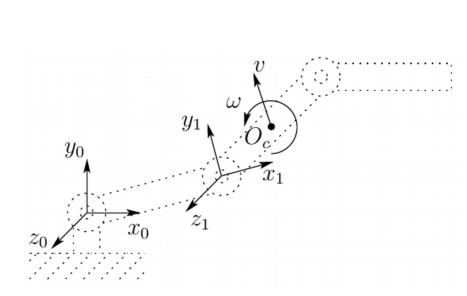
\includegraphics[width=0.6\textwidth]{q1.png}
  \caption{Three link three joint robot}
  \label{fig:q1.1}
\end{figure}
Assigning frames according to DH convention we have,
\fromlectures
\begin{figure}[h]
  \centering
  \begin{tikzpicture}[x=1cm, y=1cm, z=-0.6cm]
    % F0
    \draw [->]       (0, 0) -- (2, 0) node [right] {$x_0$};
    \draw            (0, 0) circle (0.15cm);
    \draw [fill]     (0, 0) circle (0.07cm) node [left] {$z_0$};
    % F1
    \draw [->]       (4, 2) -- (5.7888, 2.8944) node [right] {$x_1$};
    \draw            (4, 2) circle (0.15cm);
    \draw [fill]     (4, 2) circle (0.07cm) node [left] {$z_1$};
    % F1
    \draw [->]       (6, 5) -- (7.414, 6.414) node [right] {$x_2$};
    \draw            (6, 5) circle (0.15cm);
    \draw [fill]     (6, 5) circle (0.07cm) node [left] {$z_2$};
    % F3
    \draw [->]       (9, 5) -- (11, 5) node [right] {$x_3$};
    \draw            (9, 5) circle (0.15cm);
    \draw [fill]     (9, 5) circle (0.07cm) node [left] {$z_3$};
  \end{tikzpicture}
  \caption{DH frame assignment}
  \label{fig:q1.2}
\end{figure}

\begin{enumerate}[nolistsep]
  \item The z-axes are chosen along the axes of rotation.
  \item The choice of $x_0$ is free so it is chosen to be parallel to ground for simplicity.
  \item There is a unique common normal b/w $z_0$ and $z_1$, along which $x_1$ is chosen.
  \item $x_2$ and $x_3$ are chosen in the same way.
\end{enumerate}

\subsubsection*{DH parameters}
The DH parameters for the frames shown in Figure \ref{fig:q1.2} are as follows
\begin{center}
\begin{tabular}{ c | c c c c }
 \hline
 $F_i \to F_j$ & $\theta$ & d & r & $\alpha$ \\
 \hline
 $0 \to 1$ & $\theta_1$ & 0 & $l_1$ & $0^{\circ}$ \\
 $1 \to 2$ & $\theta_2$ & 0 & $l_2$ & $0^{\circ}$ \\
 $2 \to 3$ & $\theta_3$ & 0 & $l_3$ & $0^{\circ}$ \\
 \hline
\end{tabular}
\end{center}

\subsubsection*{Finding transformation $T_{03}, T_{13}, T_{23}$}
Given frame i and frame j with DH parameters [ $\theta$, d, r, $\alpha$ ] the transformation matrix is
\[
  T_{i,j} \equiv Rot_{z,\theta} * Trans_{z, d} * Trans_{x, r} * Rot_{x, \alpha}
\]
\fromlectures
Consider $T_{01}$
\[
  T_{01} \equiv Rot_{z,\theta_1} * Trans_{z, 0} * Trans_{x, l_1} * Rot_{x, 0^{\circ}}
\]
\[
  T_{01} \equiv \rz{\theta_1} * \trans{0}{0}{0} * \trans{l_1}{0}{0} * \rx{0^{\circ}}
\]
\[
  T_{01} \equiv \rz{\theta_1} * \iden * \trans{l_1}{0}{0} * \iden
\]
\[
  T_{01} \equiv \rz{\theta_1} * \trans{l_1}{0}{0}
\]
\[
  T_{01} \equiv
  \begin{bmatrix} c_1 & -s_1 & 0 & l_1c_1 \\ s_1 & c_1 & 0 & l_1s_1 \\ 0 & 0 & 1 & 0 \\ 0 & 0 & 0 & 1 \end{bmatrix}
\]
Where $c_1 \equiv cos(\theta_1), s_1 \equiv sin(\theta_1)$.
$T_{12}, T_{23}$ have the same DH-parameter structure with changed variables, therefore we can use the final form of $T_{01}$ for them.
\[
  T_{12} \equiv
  \begin{bmatrix} c_2 & -s_2 & 0 & l_2c_2 \\ s_2 & c_2 & 0 & l_2s_2 \\ 0 & 0 & 1 & 0 \\ 0 & 0 & 0 & 1 \end{bmatrix}
\]
\[
  T_{23} \equiv
  \begin{bmatrix} c_3 & -s_3 & 0 & l_3c_3 \\ s_3 & c_3 & 0 & l_3s_3 \\ 0 & 0 & 1 & 0 \\ 0 & 0 & 0 & 1 \end{bmatrix}
\]
But
\[
  T_{ij} \equiv T_{ik} * T_{kj}
\]
\fromlectures
Therefore,
\[
  T_{02} \equiv T_{01} * T_{12}
\]
\[
  T_{02} \equiv
  \begin{bmatrix} c_1 & -s_1 & 0 & l_1c_1 \\ s_1 & c_1 & 0 & l_1s_1 \\ 0 & 0 & 1 & 0 \\ 0 & 0 & 0 & 1 \end{bmatrix}
  *
  \begin{bmatrix} c_2 & -s_2 & 0 & l_2c_2 \\ s_2 & c_2 & 0 & l_2s_2 \\ 0 & 0 & 1 & 0 \\ 0 & 0 & 0 & 1 \end{bmatrix}
\]
\[
  T_{02} \equiv
  \begin{bmatrix} c_1c_2 - s_1s_2 & -(s_1c_2 + c_1s_2) & 0 & l_1c_1 + l_2(c_1c_2 - s_1s_2) \\ s_1c_2 + c_1s_2 & c_1c_2 - s_1s_2 & 0 & l_1s_1 + l_2(s_1c_2 + c_1s_2) \\ 0 & 0 & 1 & 0 \\ 0 & 0 & 0 & 1 \end{bmatrix}
\]
\[
  T_{02} \equiv
  \begin{bmatrix} c_{12} & -s_{12} & 0 & l_1c_1 + l_2c_{12} \\ s_{12} & c_{12} & 0 & l_1s_1 + l_2s_{12} \\ 0 & 0 & 1 & 0 \\ 0 & 0 & 0 & 1 \end{bmatrix}
\]
Where $c_{12} \equiv cos(\theta_1 + \theta_2), s_{12} \equiv sin(\theta_1 + \theta_2)$.
Consider $T_{03}$,
\[
  T_{03} \equiv T_{02} * T_{23}
\]
\[
  T_{03} \equiv
  \begin{bmatrix} c_{12} & -s_{12} & 0 & l_1c_1 + l_2c_{12} \\ s_{12} & c_{12} & 0 & l_1s_1 + l_2s_{12} \\ 0 & 0 & 1 & 0 \\ 0 & 0 & 0 & 1 \end{bmatrix}
  *
  \begin{bmatrix} c_3 & -s_3 & 0 & l_3c_3 \\ s_3 & c_3 & 0 & l_3s_3 \\ 0 & 0 & 1 & 0 \\ 0 & 0 & 0 & 1 \end{bmatrix}
\]
\[
  T_{03} \equiv
  \begin{bmatrix}
    c_{12}c_{3} - s_{12}s_{3} & -(s_{12}c_{3} + c_{12}s_{3}) & 0 & l_1c_1 + l_2c_{12} + l_3(c_{12}c_{3} - s_{12}s_{3})\\
    s_{12}c_{3} + c_{12}s_{3} & c_{12}c_{3} - s_{12}s_{3}    & 0 & l_1s_1 + l_2s_{12} + l_3(s_{12}c_{3} + c_{12}s_{3})\\
    0 & 0 & 1 & 0 \\
    0 & 0 & 0 & 1
  \end{bmatrix}
\]
\[
  T_{03} \equiv
  \begin{bmatrix}
    c_{123} & -s_{123} & 0 & l_1c_1 + l_2c_{12} + l_3c_{123}\\
    s_{123} & c_{123}  & 0 & l_1s_1 + l_2s_{12} + l_3s_{123}\\
    0 & 0 & 1 & 0 \\
    0 & 0 & 0 & 1
  \end{bmatrix}
\]

\subsubsection*{Finding Jacobian}
For a 3R robot, the Jacobian of pose of end effector w.r.t frame 0 as a function of joint variables
\[
  J \equiv
  \begin{bmatrix} z_0^0 \times a_{03}^0 & z_1^0 \times a_{13}^0 & z_2^0 \times a_{23}^0 \\ z_0^0 & z_1^0 & z_2^0 \end{bmatrix}
\]
where
\[
  a_{i3}^{0} \equiv a_{3}^{0} - a_{i}^{0}
\]
where $a_3^0$ is the origin of frame 3 in frame 0 and $a_i^0$ is origin of frame i in frame 0.
\fromlectures

As the robot is planar, all z-axes are in the same direction.
Therefore all z-axes in frame 0 shall have the same representation viz.
\[
  z_0^{0} \equiv z_1^{0} \equiv z_2^{0} \equiv z_3^{0} \equiv \begin{bmatrix} 0 \\ 0 \\ 1 \end{bmatrix}
\]
Consider $a_{3}^{0}$,
\[
  a_3^0 \equiv T_{03} * O_3
\]
\[
  a_3^0 \equiv
  \begin{bmatrix}
    c_{123} & -s_{123} & 0 & l_1c_1 + l_2c_{12} + l_3c_{123}\\
    s_{123} & c_{123}  & 0 & l_1s_1 + l_2s_{12} + l_3s_{123}\\
    0 & 0 & 1 & 0 \\
    0 & 0 & 0 & 1
  \end{bmatrix}
  *
  \begin{bmatrix} 0 \\ 0 \\ 0 \\ 1 \end{bmatrix}
\]
\[
  a_3^0 \equiv
  \begin{bmatrix}
    l_1c_1 + l_2c_{12} + l_3c_{123}\\
    l_1s_1 + l_2s_{12} + l_3s_{123}\\
    0 \\
    1
  \end{bmatrix}
\]
Consider $a_{2}^{0}$,
\[
  a_2^0 \equiv T_{02} * O_2
\]
\[
  a_2^0 \equiv
  \begin{bmatrix} c_{12} & -s_{12} & 0 & l_1c_1 + l_2c_{12} \\ s_{12} & c_{12} & 0 & l_1s_1 + l_2s_{12} \\ 0 & 0 & 1 & 0 \\ 0 & 0 & 0 & 1 \end{bmatrix}
  *
  \begin{bmatrix} 0 \\ 0 \\ 0 \\ 1 \end{bmatrix}
\]
\[
  a_2^0 \equiv
  \begin{bmatrix}
    l_1c_1 + l_2c_{12}\\
    l_1s_1 + l_2s_{12}\\
    0 \\
    1
  \end{bmatrix}
\]
Consider $a_{1}^{0}$,
\[
  a_1^0 \equiv T_{01} * O_1
\]
\[
  a_1^0 \equiv
  \begin{bmatrix} c_1 & -s_1 & 0 & l_1c_1 \\ s_1 & c_1 & 0 & l_1s_1 \\ 0 & 0 & 1 & 0 \\ 0 & 0 & 0 & 1 \end{bmatrix}
  *
  \begin{bmatrix} 0 \\ 0 \\ 0 \\ 1 \end{bmatrix}
\]
\[
  a_1^0 \equiv
  \begin{bmatrix}
    l_1c_1\\
    l_1s_1\\
    0 \\
    1
  \end{bmatrix}
\]
And,
\[
  a_0^0 \equiv \begin{bmatrix} 0 \\ 0 \\ 0 \\ 1 \end{bmatrix}
\]
Removing the homogeneous fourth coordinate we have,
\[
  a_0^0 \equiv
  \begin{bmatrix} 0 \\ 0 \\ 0  \end{bmatrix}
\]
\[
  a_1^0 \equiv
  \begin{bmatrix}
    l_1c_1\\
    l_1s_1\\
    0
  \end{bmatrix}
\]
\[
  a_2^0 \equiv
  \begin{bmatrix}
    l_1c_1 + l_2c_{12}\\
    l_1s_1 + l_2s_{12}\\
    0
  \end{bmatrix}
\]
\[
  a_3^0 \equiv
  \begin{bmatrix}
    l_1c_1 + l_2c_{12} + l_3c_{123}\\
    l_1s_1 + l_2s_{12} + l_3s_{123}\\
    0
  \end{bmatrix}
\]
Consider $a_{03}^0$,
\[
  a_{03}^0 \equiv a_3^0 - a_0^0
\]
\[
  a_{03}^0 \equiv
  \begin{bmatrix}
    l_1c_1 + l_2c_{12} + l_3c_{123}\\
    l_1s_1 + l_2s_{12} + l_3s_{123}\\
    0
  \end{bmatrix}
  -
  \begin{bmatrix} 0 \\ 0 \\ 0  \end{bmatrix}
\]
\[
  a_{03}^0 \equiv
  \begin{bmatrix}
    l_1c_1 + l_2c_{12} + l_3c_{123}\\
    l_1s_1 + l_2s_{12} + l_3s_{123}\\
    0
  \end{bmatrix}
\]
Consider $a_{13}^0$,
\[
  a_{13}^0 \equiv a_3^0 - a_1^0
\]
\[
  a_{13}^0 \equiv
  \begin{bmatrix}
    l_1c_1 + l_2c_{12} + l_3c_{123}\\
    l_1s_1 + l_2s_{12} + l_3s_{123}\\
    0
  \end{bmatrix}
  -
  \begin{bmatrix}
    l_1c_1\\
    l_1s_1\\
    0
  \end{bmatrix}
\]
\[
  a_{13}^0 \equiv
  \begin{bmatrix}
    l_2c_{12} + l_3c_{123}\\
    l_2s_{12} + l_3s_{123}\\
    0
  \end{bmatrix}
\]
Consider $a_{23}^0$,
\[
  a_{23}^0 \equiv a_3^0 - a_2^0
\]
\[
  a_{23}^0 \equiv
  \begin{bmatrix}
    l_1c_1 + l_2c_{12} + l_3c_{123}\\
    l_1s_1 + l_2s_{12} + l_3s_{123}\\
    0
  \end{bmatrix}
  -
  \begin{bmatrix}
    l_1c_1 + l_2c_{12}\\
    l_1s_1 + l_2s_{12}\\
    0
  \end{bmatrix}
\]
\[
  a_{23}^0 \equiv
  \begin{bmatrix}
    l_3c_{123}\\
    l_3s_{123}\\
    0
  \end{bmatrix}
\]
Consider the cross product of the form,
\[
  \begin{bmatrix} 0 \\ 0 \\ 1 \end{bmatrix} \times \begin{bmatrix} a \\ b \\ 0 \end{bmatrix}
  \equiv
  \begin{bmatrix} -b \\ a \\ 0 \end{bmatrix}
\]
Finally,
\[
  z_0^0 \times a_{03}^0 \equiv
  \begin{bmatrix} 0 \\ 0 \\ 1 \end{bmatrix} \times
  \begin{bmatrix}
    l_1c_1 + l_2c_{12} + l_3c_{123}\\
    l_1s_1 + l_2s_{12} + l_3s_{123}\\
    0
  \end{bmatrix}
  \equiv
  \begin{bmatrix}
    -(l_1s_1 + l_2s_{12} + l_3s_{123})\\
    l_1c_1 + l_2c_{12} + l_3c_{123}\\
    0
  \end{bmatrix}
\]
\[
  z_1^0 \times a_{13}^0 \equiv
  \begin{bmatrix} 0 \\ 0 \\ 1 \end{bmatrix} \times
  \begin{bmatrix}
    l_2c_{12} + l_3c_{123}\\
    l_2s_{12} + l_3s_{123}\\
    0
  \end{bmatrix}
  \equiv
  \begin{bmatrix}
    -(l_2s_{12} + l_3s_{123})\\
    l_2c_{12} + l_3c_{123}\\
    0
  \end{bmatrix}
\]
\[
  z_2^0 \times a_{23}^0 \equiv
  \begin{bmatrix} 0 \\ 0 \\ 1 \end{bmatrix} \times
  \begin{bmatrix}
    l_3c_{123}\\
    l_3s_{123}\\
    0
  \end{bmatrix}
  \equiv
  \begin{bmatrix}
    -(l_3s_{123})\\
    l_3c_{123}\\
    0
  \end{bmatrix}
\]
Using these to build the Jacobian,
\[
  J \equiv
  \begin{bmatrix}
    -(l_1s_1 + l_2s_{12} + l_3s_{123}) & -(l_2s_{12} + l_3s_{123}) & -(l_3s_{123})\\
    l_1c_1 + l_2c_{12} + l_3c_{123} & l_2c_{12} + l_3c_{123} & l_3c_{123}\\
    0 & 0 & 0 \\
    0 & 0 & 0 \\
    0 & 0 & 0 \\
    1 & 1 & 1 \\
  \end{bmatrix}
\]

\pagebreak

\section{}
\section{}
\section{}

\end{document}
